% This is a template for Ph.D. dissertations in the UCI format.
% 
% All fonts, including those for sub- and superscripts, must be 10
% points or larger.  Recommended sizes are 14-point for chapter
% headings, 12-point for the main body of text and figure/table
% titles, and 10-point for footnotes, sub- and super-scripts, and text
% in figures and tables.
%
% Notes: Add short title to figures, sections, via square brackets,
% e.g. \section[short]{long}.
%
\documentclass[12pt,fleqn]{ucithesis}

% A few common packages
\usepackage{amsmath}
\usepackage{amsthm}
\usepackage{array}
\usepackage{graphicx}
\usepackage{natbib}
\usepackage{relsize}
\usepackage[titletoc]{appendix}

% Some other useful packages
\usepackage{caption}
\usepackage{subcaption}  % \begin{subfigure}...\end{subfigure} within figure
\usepackage{multirow}
\usepackage{tabularx}
\usepackage{booktabs}

% Uncomment the following to attempt to enforce Type 1 or TrueType 
% fonts. ProQuest does not want the type 3 fonts used by default as
% of Dec. 2019 - see 
% https://support.proquest.com/articledetail?id=kA01W000000k9o2SAA . 
% If you are unable to embed fonts such as 'Zapf Dingbats' or 
% 'Symbol', try using raster images (.jpg or .png) instead of vector 
%images (.pdf or .eps).
% \usepackage[T1]{fontenc} 

% plainpages=false fixes the "duplicate ignored" error with page counters
% Set pdfborder to 0 0 0 to disable colored borders around PDF hyperlinks
\usepackage[plainpages=false,pdfborder={0 0 0}]{hyperref}

% Uncomment the following line to use the algorithm package,
% which provides an algorithm environment similar to figure and table
% ("\begin{algorithm}...\end{algorithm}"). A list of algorithms will
% automatically be added in the preliminary pages. Note that you
% probably want a package for the actual code to go with this (e.g.,
% algorithmic).
%\usepackage{algorithm}

% Uncomment the following line to enable Unicode support. This will allow you
% to enter non-ASCII characters (such as accented characters) directly without
% having to use LaTeX's awkward escape syntax (e.g., \'{e})
% NOTE: You may have to install the ucs.sty package for this to work. See:
% http://www.unruh.de/DniQ/latex/unicode/
%\usepackage[utf8x]{inputenc}

% Uncomment the following to avoid "widowing", where page breaks cause
% single lines of paragraphs to float onto the next page (this is not
% a UCI requirement but more of an aesthetic choice).
%\widowpenalty=10000
%\clubpenalty=10000

% Modify or extend these at will.
\newtheorem{theorem}{\textsc{Theorem}}[chapter]
\newtheorem{definition}{\textsc{Definition}}[chapter]
\newtheorem{example}{\textsc{Example}}[chapter]

% My macros
\newcommand{\pkg}[1]{\texttt{#1}}
\newcommand\elec{\mathrm{e^-}}

% Macros for title, author, abstract, etc.
\thesistitle{Title of the Thesis}

%"Dissertation" for PhD, "Thesis" for master's
\documenttitle{Dissertation}

\degreename{Doctor of Philosophy}

% Use the wording given in the official list of degrees awarded by UCI:
% http://www.rgs.uci.edu/grad/academic/degrees_offered.htm
\degreefield{Physics \& Astronomy}

% Your name as it appears on official UCI records.
\authorname{Bela Abolfathi}

% Use the full name of each committee member and full title 
% (e.g. Professor/Associate Professor).
\committeechair{Professor David P. Kirkby}
\othercommitteemembers
{
  Associate Professor Simona Murgia\\
  Professor Mu-Chun Chen
}

\degreeyear{2021}

\copyrightdeclaration
{
  {\copyright} {\Degreeyear} \Authorname
}

% If you have previously published parts of your manuscript, you must list the
% copyright holders; see Section 3.2 of the UCI Thesis and Dissertation Manual.
% Otherwise, this section may be omitted.
% \prepublishedcopyrightdeclaration
% {
% 	Chapter 4 {\copyright} 2003 Springer-Verlag \\
% 	Portion of Chapter 5 {\copyright} 1999 John Wiley \& Sons, Inc. \\
% 	All other materials {\copyright} {\Degreeyear} \Authorname
% }

% The dedication page is optional
% (comment out to exclude).
\dedications
{
  (Optional dedication page)
  
  To ...
}

\acknowledgments
{
  I would like to thank...
  
  (You must acknowledge grants and other funding assistance. 
  
  You may also acknowledge the contributions of professors and
  friends.
  
  You also need to acknowledge any publishers of your previous
  work who have given you permission to incorporate that work
  into your dissertation. See Section 3.2 of the UCI Thesis and
  Dissertation Manual.)
}


% Some custom commands for your list of publications and software.
\newcommand{\mypubentry}[3]{
  \begin{tabular*}{1\textwidth}{@{\extracolsep{\fill}}p{4.5in}r}
    \textbf{#1} & \textbf{#2} \\ 
    \multicolumn{2}{@{\extracolsep{\fill}}p{.95\textwidth}}{#3}\vspace{6pt} \\
  \end{tabular*}
}
\newcommand{\mysoftentry}[3]{
  \begin{tabular*}{1\textwidth}{@{\extracolsep{\fill}}lr}
    \textbf{#1} & \url{#2} \\
    \multicolumn{2}{@{\extracolsep{\fill}}p{.95\textwidth}}
    {\emph{#3}}\vspace{-6pt} \\
  \end{tabular*}
}

% Include, at minimum, a listing of your degrees and educational
% achievements with dates and the school where the degrees were
% earned. This should include the degree currently being
% attained. Other than that it's mostly up to you what to include here
% and how to format it, below is just an example.
%
% CV is required for PhD theses, but not Master's
% comment out to exclude
\curriculumvitae
{

\textbf{EDUCATION}
  
  \begin{tabular*}{1\textwidth}{@{\extracolsep{\fill}}lr}
    \textbf{Doctor of Philosophy in Physics \& Astronomy} & \textbf{2021} \\
    \vspace{6pt}
    University of California, Irvine & \emph{Irvine, CA} \\
    \textbf{Master of Science in Physics \& Astronomy} & \textbf{2016} \\
    \vspace{6pt}
    University of California, Irvine & \emph{Irvine, CA} \\
    \textbf{Bachelor of Arts in Physics} & \textbf{2011} \\
    \vspace{6pt}
    Reed College & \emph{Portland, OR} \\
  \end{tabular*}

\vspace{12pt}
\textbf{RESEARCH EXPERIENCE}

  \begin{tabular*}{1\textwidth}{@{\extracolsep{\fill}}lr}
    \textbf{Graduate Student Researcher} & \textbf{2014-2021} \\
    \vspace{6pt}
    University of California, Irvine & \emph{Irvine, California} \\
    \textbf{Graduate Student Researcher} & \textbf{2018} \\
    \vspace{6pt}
    SLAC National Accelerator Laboratory & \emph{Menlo Park, CA} \\
    \textbf{REU Student} & \textbf{Summer 2010} \\
    \vspace{6pt}
    Cornell University & \emph{Ithaca, New York} \\
  \end{tabular*}

\vspace{12pt}
\textbf{TEACHING EXPERIENCE}

  \begin{tabular*}{1\textwidth}{@{\extracolsep{\fill}}lr}
    \textbf{Teaching Assistant} & \textbf{2014--2016} \\
    \vspace{6pt}
    University of California, Irvine & \emph{Irvine, California} \\
  \end{tabular*}

\pagebreak

\textbf{REFEREED JOURNAL PUBLICATIONS}

  \mypubentry{DC2 Paper}{TBD}{Journal name}
  \mypubentry{Overview of the DESI Legacy Imaging Surveys}{2018}{Astronomical Journal}
  \mypubentry{The Fourteenth Data Release of the Sloan Digital Sky Survey}{2018}{Astrophys. J., Suppl}
  \mypubentry{Sloan Digital Sky Survey IV: Mapping the Milky Way, Nearby Galaxies, and the Distant Universe}{2017}{Astronomical Journal}
  \mypubentry{Discovery and Follow-up Observations of the Young Type Ia Supernova 2016coj}{2017}{Astrophysical Journal}

%\vspace{12pt}
%\textbf{REFEREED CONFERENCE PUBLICATIONS}

  %\mypubentry{Awesome paper}{Jun 2011}{Conference name}
  %\mypubentry{Another awesome paper}{Aug 2012}{Conference name}

\vspace{12pt}
\textbf{SOFTWARE}

  \mysoftentry{pz\_bayes}{http://your.url.here/}
  {C++ algorithm that solves TSP in polynomial time.}

}

% The abstract was previously limited to a maximum of 350 words, 
% but the UCI manual at https://etd.lib.uci.edu/electronic/td2e#2.2.1.
% currently does not indicate that there is any word limit for the abstract
\thesisabstract
{
  The abstract of your contribution goes here.
}


%%% Local Variables: ***
%%% mode: latex ***
%%% TeX-master: "thesis.tex" ***
%%% End: ***


% Add PDF document info fields
\hypersetup{
	pdftitle={\Thesistitle},
	pdfauthor={\Authorname},
	pdfsubject={\Degreefield},
}


% Uncomment the following to have numbered subsubsections (by default
% numbering goes only to subsections).
%\setcounter{secnumdepth}{4}

% Set this to only select a subset of the includes directives below.
% Very handy to speed up compilation if you're working on a certain
% part of your thesis. It conserves page numbers, references, etc.
% even for non-included files.
%\includeonly{chapter1}

\begin{document}

% Preliminary pages are always loaded (TOC, CV, etc.)
\preliminarypages

% Include the different components of your thesis, in separate files.
% Using \include allows you to set \includeonly above.
\chapter{Introduction}

This is an example using the \LaTeX{} template for UCI theses and
dissertation documents \cite{uci-thesis-latex}. Figure
\ref{fig:sourcecode} is just for illustration purposes, as is Table
\ref{tab:coordinates}.

\begin{figure}
\begin{verbatim}
#include <iostream>
int main(int argc, char** argv) {
  std::cout << "Hello World." << std::endl;
  return 0;
}
\end{verbatim}
  \caption{Example source code.}
  \label{fig:sourcecode}
\end{figure}

\section{Background}

Lorem ipsum dolor sit amet, consectetur adipisicing elit, sed do
eiusmod tempor incididunt ut labore et dolore magna aliqua. Ut enim ad
minim veniam, quis nostrud exercitation ullamco laboris nisi ut
aliquip ex ea commodo consequat. Duis aute irure dolor in
reprehenderit in voluptate velit esse cillum dolore eu fugiat nulla
pariatur. Excepteur sint occaecat cupidatat non proident, sunt in
culpa qui officia deserunt mollit anim id est laborum.

\begin{table}
  \centering
  \begin{tabular}{|rr|r|}
    \hline
    $x$ & $y$ & $z$ \\
    \hline
    14 & 12 & -2 \\
    0 & 33 & -25 \\
    -3 & 11 & 22 \\
    4 & 4 & 6 \\
    \hline
  \end{tabular}
  \caption{Example coordinates.}
  \label{tab:coordinates}
\end{table}

Lorem ipsum dolor sit amet, consectetur adipisicing elit, sed do
eiusmod tempor incididunt ut labore et dolore magna aliqua. Ut enim ad
minim veniam, quis nostrud exercitation ullamco laboris nisi ut
aliquip ex ea commodo consequat. Duis aute irure dolor in
reprehenderit in voluptate velit esse cillum dolore eu fugiat nulla
pariatur. Excepteur sint occaecat cupidatat non proident, sunt in
culpa qui officia deserunt mollit anim id est laborum.

\section{History}
\section{Dark energy}
\section{Theoretical framework}
\section{Stage IV Dark Energy Experiments}
\subsection{Vera C. Rubin Observatory}
\subsection{Dark Energy Spectroscopic Instrument}
\section{Observational probes}
\subsection{Weak gravitational lensing}
\subsection{BAO in the Lyman-$\alpha$ forest of high redshift quasars}
\section{Motivation and results}
% talk about requirements here (both in terms of image quality and electrical)
% linearity requirements are motivated by requirements on photometric accuracy

%%% Local Variables: ***
%%% mode: latex ***
%%% TeX-master: "thesis.tex" ***
%%% End: ***

\chapter{Redshift inference using a hierarchical Bayesian model}



%%% Local Variables: ***
%%% mode: latex ***
%%% TeX-master: "thesis.tex" ***
%%% End: ***

\chapter{Sensor effects}

\section{Modeling sky brightness in the ImSim package}
\section{Simulating the brighter-fatter effect}
\section{Bias and offset corrections in LSST sensors}




%%% Local Variables: ***
%%% mode: latex ***
%%% TeX-master: "thesis.tex" ***
%%% End: ***

\chapter{Magnitude and shape distributions for mock selection of DESI targets}

\section{DESI Target selection}

%https://doi.org/10.3847/1538-3881/ab089d
%https://ui.adsabs.harvard.edu/abs/2013AJ....145...10D/abstract
%https://academic.oup.com/mnras/article/455/2/1553/1112409#92067589
% CLASS = TARGET TYPE?
% What tense should this be in - past or present?
% Make comparison to eBOSS?
% Describe cuts made on the data
% Include description of each shape profile
% Include description of density contours for 2D Gaussian
% There is noticable difference between my results and John's albeit he used different cuts - could this be due to the cuts, but also because he is running the GMMs on DR 7.1? Did Tractor calculation of fluxes improve in subsequent data releases?

DESI will extract spectra from over 35 million astrophysical sources to measure the expansion rate over the past 11 billion years. To do this it will need an inventory of targets to choose from so that it can know where to point its 5,000 optical fibers. DESI pre-selected targets to observe from three separate imaging surveys, collectively referred to as the DESI Legacy Imaging Surveys. These wide-field surveys will provide photometry that is both uniform and spatially dense, ultimately pushing to depths around 2 magnitudes deeper than SDSS.  Compared to SDSS, the Legacy Surveys will detect over 15 times the number of $z>0.5$ galaxies and over 200 times more $z>1.0$ galaxies by reaching $5\sigma$ depth in the z-band (Dey et. al Overview). The utility of these surveys goes beyond target selection for DESI, as they can be used in tandem with overlapping spectroscopic data in a variety of contexts such as redshift estimation through the use of spectroscopic priors or to study dark matter halos by cross-correlating spectroscopic and imaging maps (Dey et. al Overview).

\subsection{DESI Legacy Imaging Surveys}

The Legacy Surveys completely overlap with DESI's approximately 14000 deg$^2$ footprint, which is divided into separate 9900 deg$^2$ and 4000 deg$^2$ patches in each of the Northern and Southern Galactic Caps, respectively (Fig. \ref{fig:footprint}). The Dark Energy Camera (DECam, Flaugher et al 2015), which is installed on the 4-meter Blanco telescope at the Cerro Tololo Inter-American Observatory, imaged the entire SGC footprint and part of the NGC in $g,r,z$ bands as part of the Dark Energy Camera Legacy Survey (DECaLS). The majority of DESI's northern footprint was imaged at Kitt Peak National Observatory. Photometry in the $g$- and $r$-bands was taken by the Prime90 instrument on the Bok Telescope as part of the Beijing-Arizona Sky Survey (BASS, Zou et al 2017b), and additional $z$-band photometry was provided by the Mayall z-band Legacy Survey (MzLS) which used the Mosaic-3 camera on the Mayall 4-meter Telescope. These optical data were combined with mid-infrared photometry from the Wide-field Infrared Survey Explorer (WISE) satellite (ref) to help differentiate between targets and characterize morphology, and was particularly useful for selecting luminous red galaxies and quasars. See Table \ref{tab:legacy} for more info about survey coverage and depths. (Might want to include Table 1 and/or Table 2 from Dey et. al)

\begin{figure}\centering
\subfloat[g-band]{\label{a}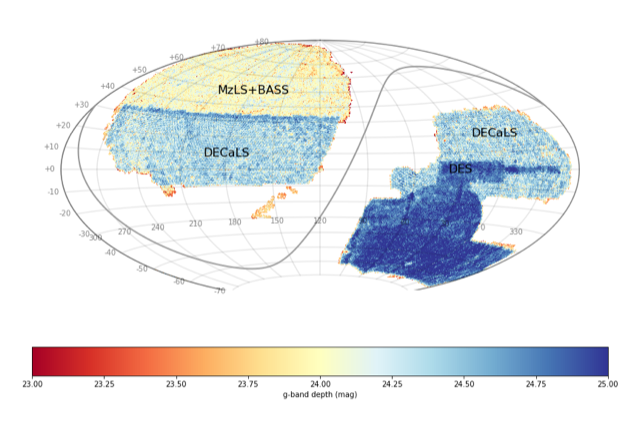
\includegraphics[width=.45\linewidth]{images/gmm/depth-g-dr9.png}}\hfill
\subfloat[r-band]{\label{b}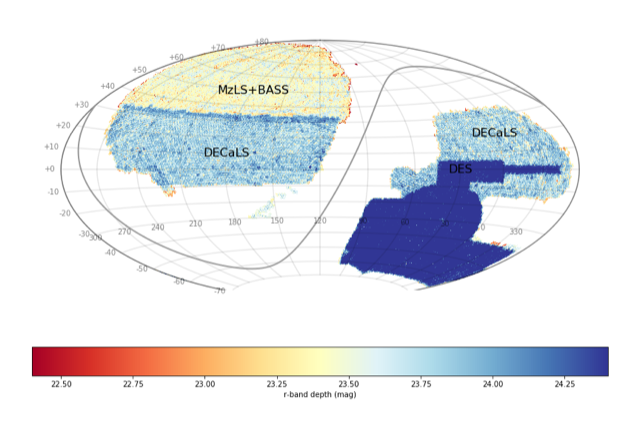
\includegraphics[width=.45\linewidth]{images/gmm/depth-r-dr9.png}}\par 
\subfloat[z-band]{\label{c}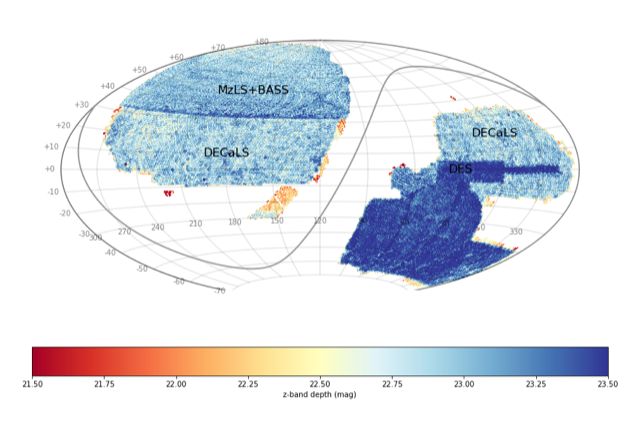
\includegraphics[width=.45\linewidth]{images/gmm/depth-z-dr9.png}}
\caption{DR9 footprint. Credit: https://www.legacysurvey.org/status/}
\label{fig:footprint}
\end{figure}


% Fix the qsos in the table so that number and z range are split for the same class
\begin{table}
\caption{DESI Legacy Surveys: Areas and Depths}
\label{tab:legacy}
\centering
\begin{tabular}{c c c c c}
\toprule
\multicolumn{4}{c}{xxx xx xxxx}   \\
\midrule
  \hline
  \hline
  Survey Name & Telescope/Instrument & Galaxy Depth (mag) & Area (deg$^2$) & Location\\
  \hline \hline
  DECaLS & \begin{tabular}{c|c|c}
  g & r & z\\
  \hline
  23.72 & 23.27 & 22.22 \\
  \end{tabular}
  & 9000 \\
  \hline
  BASS & \begin{tabular}{c|c}
  g & r \\
  \hline
  23.48 & 22.87 &  \\
  \end{tabular} & 5000 \\
  \hline
  MzLS & \begin{tabular}{c}
  z\\
  \hline
   &  &  22.29\\
  \end{tabular} & 5000 \\
  \hline
\end{tabular}
%Median 5$\sigma$ detection limit in AB mag for the fiducial DESI target 
%Add WISE info?
\end{table}\\

\subsection{Target classes}
%sources from: https://www.desi.lbl.gov/2020/11/04/desi-target-selection/

DESI will observe luminous red galaxies (LRG), emission line galaxies (ELG), quasars (QSO) and bright galaxies (BGS), to study cosmic expansion and the growth rate of structure using baryonic acoustic oscillations (BAO) and redshift space distortions (RSD). Fainter, higher-redshift targets such as LRGs, ELGs, and QSOs will be observed during a Dark Time Program, when there is little light contamination from the moon. Low redshift BGS targets will fall under the Bright Time Program, as they will be able to achieve DESI's signal-to-noise requirements despite significant moon illumination.

During its Bright Galaxy Survey, DESI will obtain spectra of 10 million low redshift galaxies below $z<0.4$ to study BAO and RSD via galaxy clustering. At slightly higher redshifts, between $0.3<z<1.0$, it will target at least 8 million LRGs. These galaxies are characterized by a strong $4000\mbox{\AA}$ break, a signature of the absorption of high energy radiation by metals in cooler stellar atmospheres that have ceased star formation. ELGs will comprise at least half of all DESI targets. These bluer, star-forming galaxies will probe the $0.6<z<1.6$ universe and will reveal identifiable emission lines such as the OII doublet. 
%will ELGs and LRGs be used for BAO and RSD as well?
Finally, DESI will target QSOs in an even higher redshift regime. QSOs that lie between $0.9<z<2.1$ will be used as direct tracers of dark matter, and beyond $z>2.1$, ``Lyman-alpha" quasars will study large scale structure through the absorption of neutral hydrogen in the intergalactic medium. Table \ref{tab:targets} shows each class alongside the redshift regime in which it was targeted.

%https://arxiv.org/pdf/1901.01581.
%https://indico.in2p3.fr/event/18819/contributions/71674/attachments/53296/69308/TS_SV_Desi_ChY.pdf
\begin{table}
\caption{DESI target classes.}
\label{tab:targets}
\centering
\begin{tabular}{|c|c|c|}
  \hline
  Class & Number & Redshift range\\
  \hline \hline
  BGS & 10 million & $0.05<z<0.4$ \\
  \hline
  LRG & 4 million & $0.4<z<1.0$ \\
  \hline
  ELG & 17.1 million & $0.6<z<1.7$ \\
  \hline
  QSO & 1.7 million & $0.9<z<2.1$ \\
  \hline
  QSO & 0.7 million & $z>2.1$\\
  \hline
\end{tabular}
\end{table}\\

Objects from these target classes are selected from the imaging surveys based on their specific photometric properties. After reduction with the \pkg{legacypipe} pipeline, the \pkg{desitarget} package was used to select targets from the processed images. Targets were selected based on a set of unique magnitude and color cuts that captured distinguishing features of each class. The baseline fiducial cuts for each class of object are shown in Tables \ref{tab:lrg_cuts}-\ref{tab:qso_cuts}. The resulting target catalogs were compiled in the form of data releases. The studies in this chapter were performed on imaging from Data Release 5 (DR5).


%https://desi.lbl.gov/trac/wiki/TargetSelectionWG 
\begin{table}
\caption{LRG selection cuts North}
\label{tab:lrg_cuts}
\centering
\begin{tabular}{|c|c|c|}
  \hline
  Selection & North\\
  \hline \hline
  Non-stellar cut & (z - W1) $>$ 0.8 \times \,(r - z) - 0.6 \\
  \hline
  Faint limit & zfiber $<$ 21.5 \\
  \hline
  Low-z cut & ((g - W1 $>$ 2.67) AND (g - r $>$ 1.45)) OR (r - W1 $>$ 1.85) \\
  \hline
  Double sliding cuts & (r - z $>$ (z - 16.79) $\times$ \,0.45) AND (r - z $>$ (z - 13.76) $\times$ \,0.19)
 \\
  \hline
\end{tabular}
\end{table}\\
%% zfiber? fiber magnitude vs ???

\begin{table}
\caption{LRG selection cuts South}
\label{tab:lrg_cuts}
\centering
\begin{tabular}{|c|c|c|}
  \hline
  Selection & South\\
  \hline \hline
  Non-stellar cut & (z - W1) $>$ 0.8 \times \,(r - z) - 0.6 \\
  \hline
  Faint limit & zfiber $<$ 21.5 \\
  \hline
  Low-z cut & ((g - W1 $>$ 2.6) AND (g - r $>$ 1.4)) OR (r - W1 $>$ 1.8) \\
  \hline
  Double sliding cuts & (r - z $>$ (z - 16.83) $\times$ \,0.45) AND (r - z $>$ (z - 13.80) $\times$ \,0.19) \\
  \hline
\end{tabular}
\end{table}\\

\begin{table}
\caption{ELG selection cuts}
\label{tab:elg_cuts}
\centering
\begin{tabular}{|c|c|c|}
  \hline
  Selection & North & South\\
  \hline \hline
  Bright cut & g $>$ 20.0 \\
  \hline
  Faint cut & g$<$23.5 & g$<$23.4 \\
  \hline
  Blue cut & rz$>$0.3 \\
  \hline
  Red cut & rz$<$1.6 \\
  \hline
  Star/low-z cut & gr$<$1.15\times \,rz-0.20 & gr$<$1.15 \times \,rz-0.15 \\
  \hline
  OII & gr$<$-1.20 \times \,rz+1.6 \\
  \hline
\end{tabular}
\end{table}\\

\begin{table}
\caption{QSO selection cuts}
\label{tab:qso_cuts}
\centering
\begin{tabular}{|c|c|c|}
  \hline
  Selection & North & South\\
  \hline \hline
   & 17.5 $<$ r $<$ 22.7  \\
  \hline
   & grz $>$ 17.0  \\
  \hline
   & (g-r) $<$ 1.3 \\
  \hline
   & -0.4 $<$ (r-z) $<$ 1.1 \\
  \hline
   & W1-W2 $>$ -0.3 & W1-W2 $>$ -0.4\\
  \hline
\end{tabular}
\end{table}\\

\section{Generating inputs for mocks}
%https://www.legacysurvey.org/dr9/description/
Aside from target selection, another use for these imaging catalogues is to generate realistic synthetic spectra, or mocks. DESI used the \pkg{desisim} software to simulate DESI-like spectra for a variety of purposes, including identifying and accounting for systematics, testing science pipelines, and survey strategy and design. \pkg{desisim} uses a function called \pkg{select\_mock\_targets} to randomly assign fluxes and shapes to galaxies based on representative distributions of those features. I generated flux and shape distributions for \pkg{select\_mock\_targets} using mixtures of Gaussians to characterize each target class that passed selection cuts. These models were stored as \pkg{.fits} files in \pkg{desitarget} and sampled from using \pkg{desisim}.

%https://github.com/desihub/desitarget/issues/106

\subsection{Gaussian mixture models}

% should I go into the math behind GMMs here?

A mixture model is a form of density estimation that can be used to create generative models of multi-dimensional data. This is done by assuming that the data come from a mixture of components, or Gaussians, whose parameters are optimized using an expectation-maximization (EM) algorithm. The model is then used to assign probabilities to an input vector belonging to a given component. 

\subsection{Model selection}

Gaussian mixture models are useful in characterizing sub-populations within a data set in order to generate new random data that resembles the input data. Properties of the data set are learned through training a number of models with a varying number of components in an unsupervised way. The optimal number of components in the model is determined based on a combination of model complexity (the number of degrees of freedom or components in the model) and model performance (a maximum-likelihood estimate of the data given the model). A common model selection process is the Bayesian Information Criterion (BIC), which is expressed analytically as

\begin{equation}
    BIC = k\,\ln{n} - 2\,\ln\hat{L},
\end{equation}

where $k$ is the number of model parameters, $n$ is the sample size, and $\ln\hat{L}$ is the maximum log-likelihood of the model. The model parameters for a GMM are the means and covariances of the Gaussian components. Once the BIC is evaluated for a set of models, the model with the lowest BIC is selected as the most optimal. Flux and shape distributions were generated using a Gaussian mixture model with the optimal number of components given by the minimum BIC. 

\subsection{Flux and shape distributions in DR 5}

 Rather than model sizes, shapes, colors and magnitudes simultaneously, colors and magnitudes were modeled separately for each morphological type (why did we decide to do it this way? lower-dimensional Gaussians/fewer components?). Morphological classifications were assigned according to each target's surface brightness profile, as inferred by the Tractor fitting algorithm (cite). The morphological types used in DR5 are point sources (PSF), round exponential galaxies with a variable radius (REX), deVaucouleurs profiles (DEV), exponential profiles (EXP), and composite profiles (COMP), which are a combination of deVaucouleurs and exponential profiles. Table \ref{tab:morph} shows the distribution of types in DR5 in the absence of selection cuts, and the plots in Fig. \ref{fig:morphfrac} show the fraction of targets belonging to each morphological classification in ten bins equally spaced in magnitude.

\begin{table}
\caption{Morphological types in DR5.}
\label{tab:morph}
\centering
\begin{tabular}{|c|c|}
  \hline
  Type & Number of sources\\
  \hline \hline
   PSF & 371,088,269 \\
  \hline
   REX & 222,184,611 \\
  \hline
   DEV & 22,036,854 \\
  \hline
   EXP & 61,380,049 \\
  \hline
   COMP & 3,066,121	\\
  \hline
\end{tabular}
\end{table}\\


\begin{figure}
\begin{subfigure}{.5\textwidth}
\centering
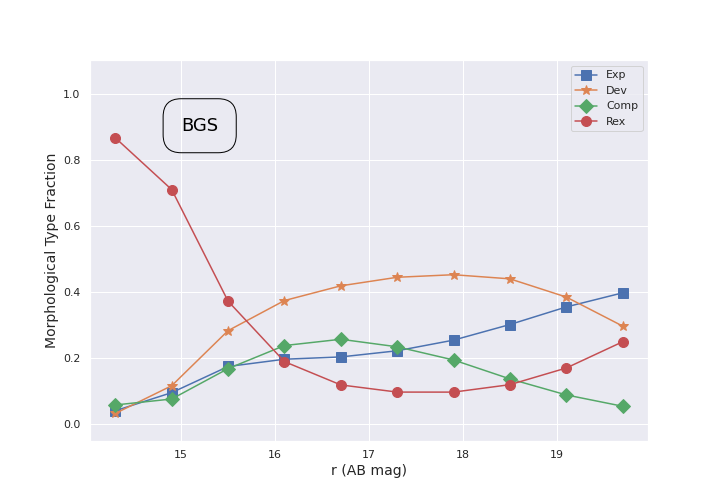
\includegraphics[width=1\linewidth]{images/gmm/bgs_morph.png}
\caption{}
\end{subfigure}
\hfill
\begin{subfigure}{.5\textwidth}
\centering
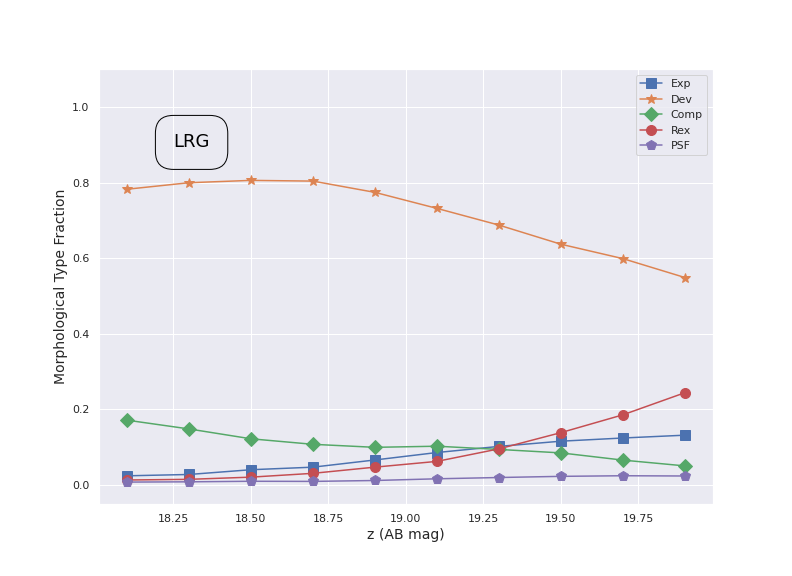
\includegraphics[width=1\linewidth]{images/gmm/lrg_morph.png}
\caption{}
\end{subfigure}
\hfill
\begin{subfigure}{.5\textwidth}
\centering
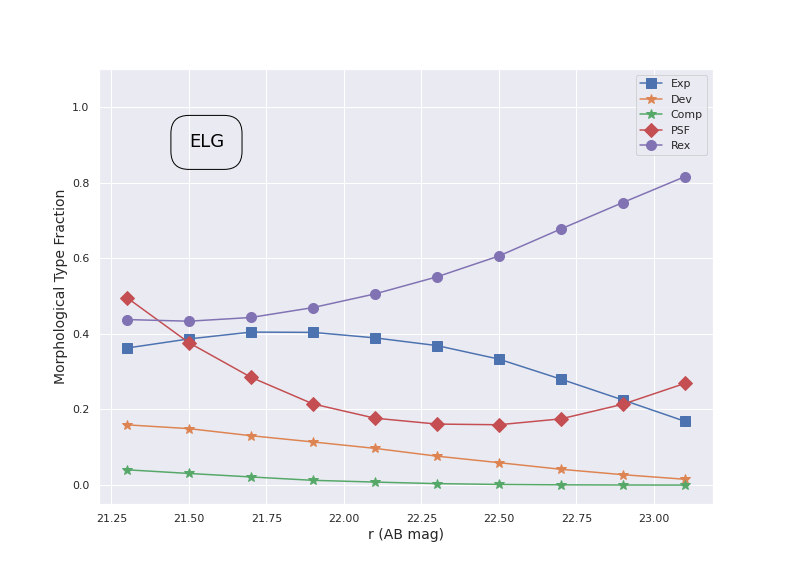
\includegraphics[width=1\linewidth]{images/gmm/elg_morph.png}
\caption{}
\end{subfigure}
\begin{subfigure}{.5\textwidth}
\centering
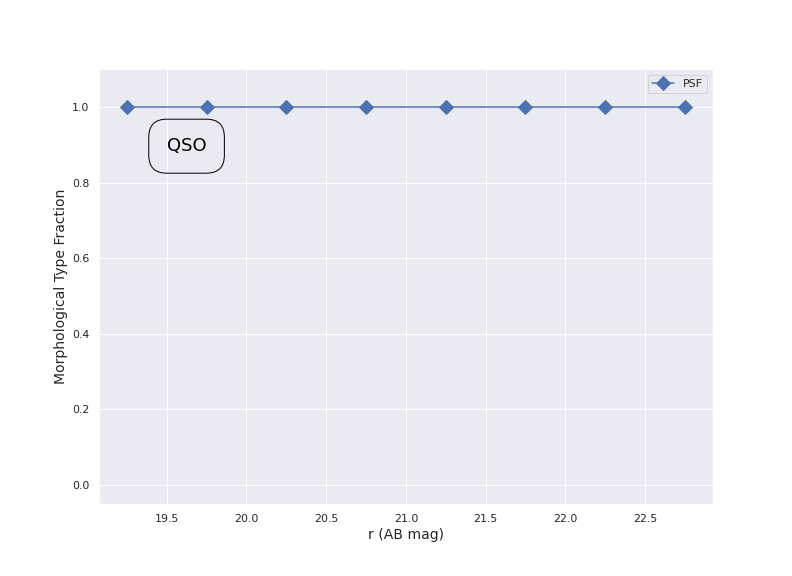
\includegraphics[width=1\linewidth]{images/gmm/qso_morph.png}
\caption{}
\end{subfigure}
\label{fig:morphfrac}
\caption{Morphological type fraction.}
\end{figure}

The features used to build the GMMs were based on the magnitudes and colors used in the selection cuts for each class. GMMs were first trained on the photometry, and then the model parameters and weights were used to generate synthetic distributions of the data with the same features. The data were split into a training set used to train the model, and a validation set used to assess the performance of the model on data that were not used for training. 


The results in Fig. \ref{} are the 2-dimensional histograms for a subset of the 

this process was extended in a similar fashion for the remaining combinations of classes and morphologies. 


(Describe training/test/validation process?)



\begin{figure}
  \centering
  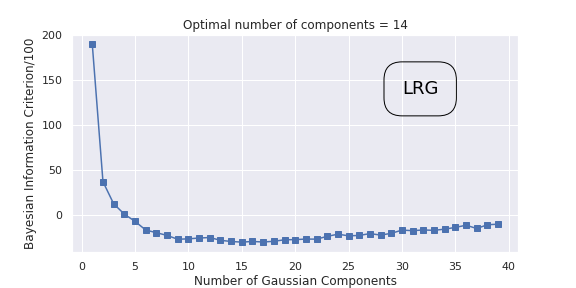
\includegraphics[width=\textwidth]{images/gmm/lrgDev_bic.png}
  \caption{LRGs.}
  \label{fig:lrg_bic}
\end{figure}

\begin{figure}
\centering
\begin{subfigure}[b]{.5\textwidth}
  \centering
  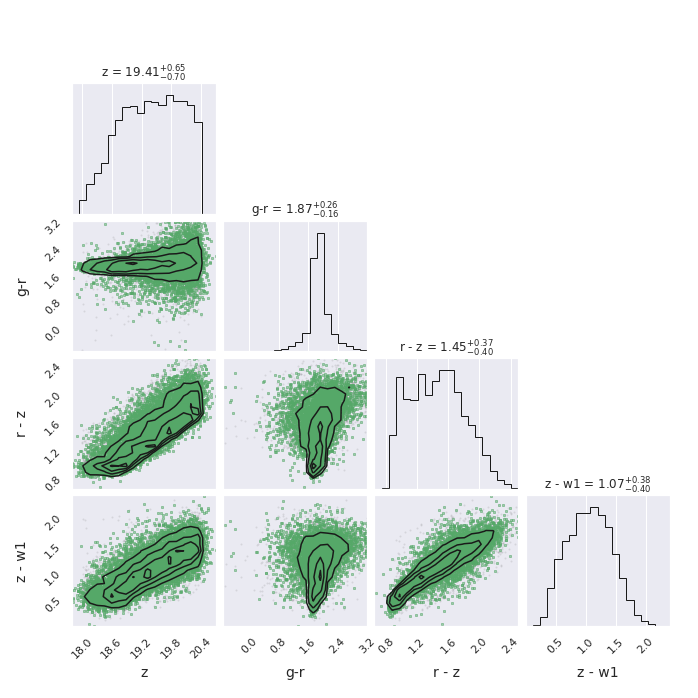
\includegraphics[width=\textwidth]{images/gmm/lrgDev_training.png}
  \caption{Training.}
  \label{fig:lrg_train}
\end{subfigure}%
\begin{subfigure}[b]{.5\textwidth}
  \centering
  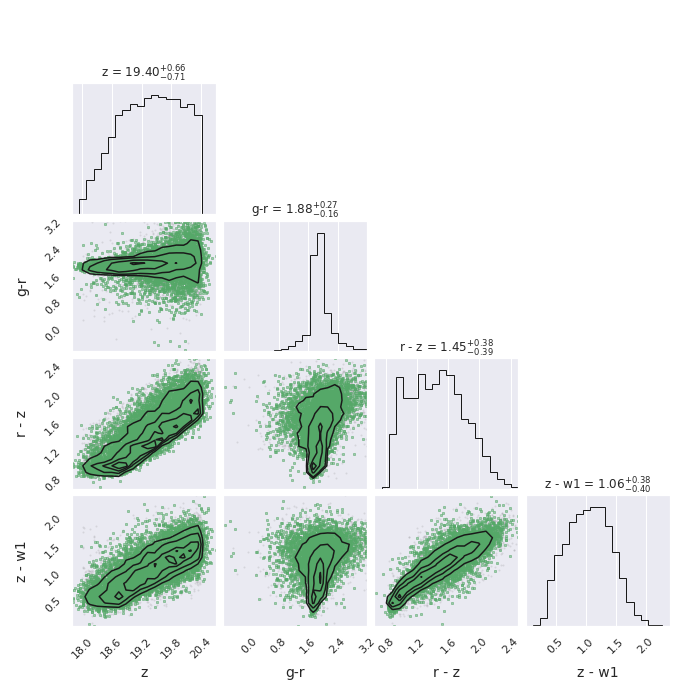
\includegraphics[width=\textwidth]{images/gmm/lrgDev_valid.png}
  \caption{Valid.}
  \label{fig:lrg_valid}
\end{subfigure}
\caption{Train/sampled/val for LRGs.}
\label{fig:lrg_gmm}
\end{figure}



\begin{figure}
  \centering
  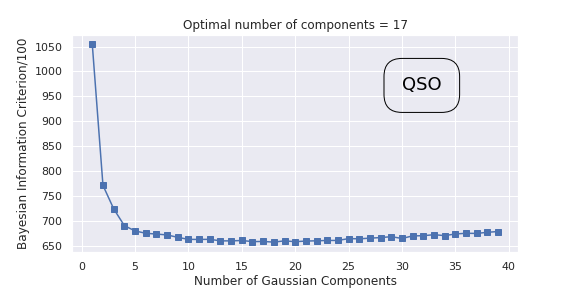
\includegraphics[width=\textwidth]{images/gmm/qso_bic.png}
  \caption{QSOs.}
  \label{fig:qso_bic}
\end{figure}

\begin{figure}
\centering
\begin{subfigure}[b]{.5\textwidth}
  \centering
  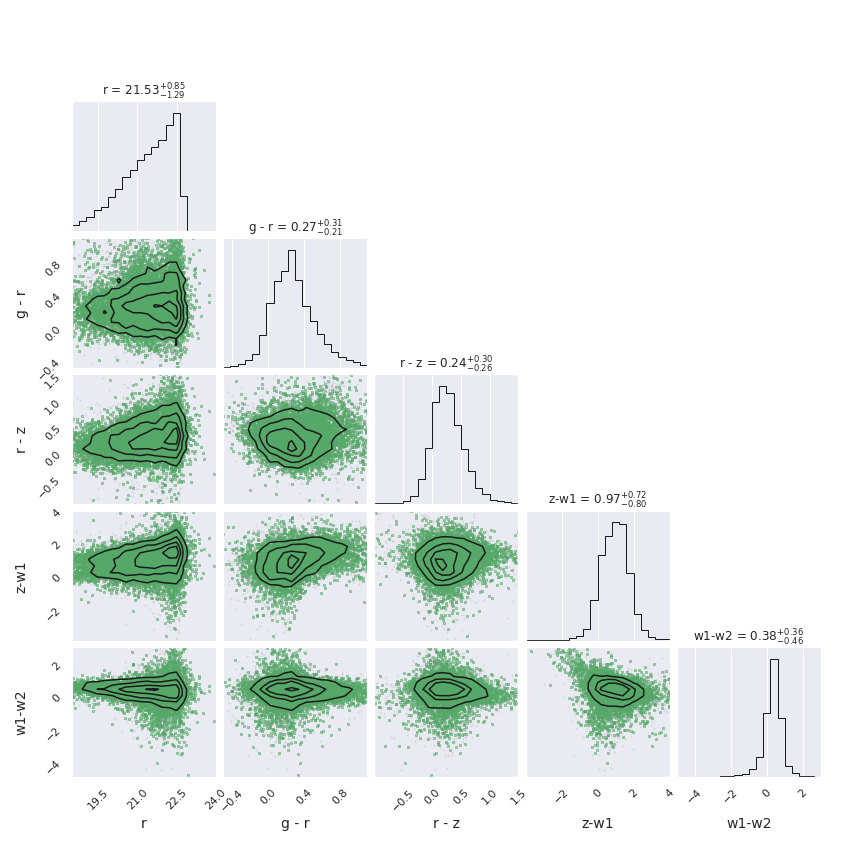
\includegraphics[width=\textwidth]{images/gmm/qso_training.png}
  \caption{Training.}
  \label{fig:qso_train}
\end{subfigure}%
\begin{subfigure}[b]{.5\textwidth}
  \centering
  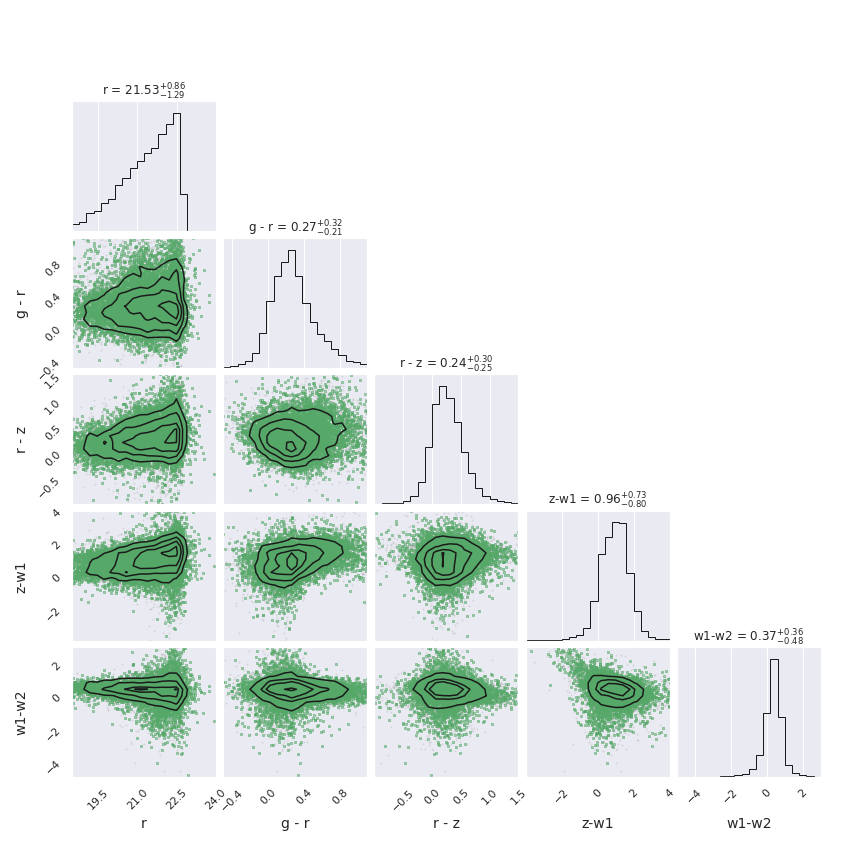
\includegraphics[width=\textwidth]{images/gmm/qso_valid.png}
  \caption{Valid.}
  \label{fig:lrg_valid}
\end{subfigure}
\caption{Train/sampled/val for QSOs.}
\label{fig:qso_gmm}
\end{figure}



\subsection{Extreme Deconvolution}




%%% Local Variables: ***
%%% mode: latex ***
%%% TeX-master: "thesis.tex" ***
%%% End: ***

\chapter{Reconfiguring the specsim package to simulate the DESI instrument}




%%% Local Variables: ***
%%% mode: latex ***
%%% TeX-master: "thesis.tex" ***
%%% End: ***

\chapter{Survey validation}



%%% Local Variables: ***
%%% mode: latex ***
%%% TeX-master: "thesis.tex" ***
%%% End: ***

% ... and so on

% These commands fix an odd problem in which the bibliography line
% of the Table of Contents shows the wrong page number.
\clearpage
\phantomsection

% "References should be formatted in style most common in discipline",
% abbrv is only a suggestion.
\bibliographystyle{abbrv}
\bibliography{thesis}

% The Thesis Manual says not to include appendix figures and tables in
% the List of Figures and Tables, respectively, so these commands from
% the caption package turn it off from this point onwards. If needed,
% it can be re-enabled later (using list=yes argument).
\captionsetup[figure]{list=no}
\captionsetup[table]{list=no}

% If you have an appendix, it should come after the references.
\begin{appendices}
\include{appendix}
\end{appendices}

\end{document}
